\subsubsection{Set 2 - Lindemans Aalst}
\label{sec:PL1_Aalst2}
% TODO: vergelijking
% TODO: andere stats ook bijzetten
\begin{figure}
  \centering
  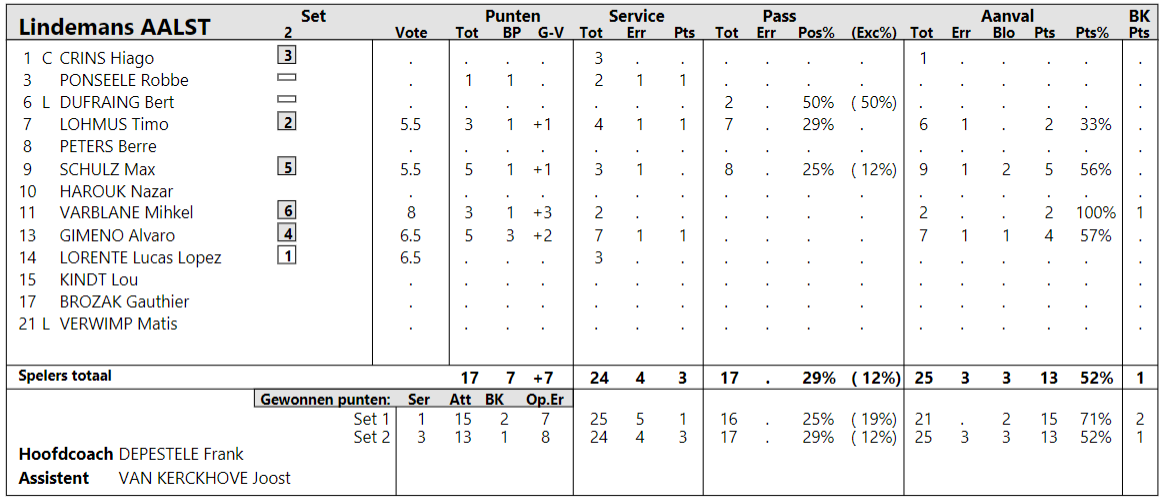
\includegraphics[width=\textwidth]{PL1_AM/SET2/PL1_AM_2.png}
  \caption{\label{fig:PL1_AM_2}Resultaten van de manuele invoer van Lindemans Aalst in set 2.}
\end{figure}

\begin{table}[ht!]
  \centering
  \scriptsize
  \begin{tabular}{|l|c|c|c|c|c|c|c|c|c|c|c|c|} \hline
    \textbf{Name} & SA & SE & TA & Pct & Eff & Rtg & 0 & 1 & 2 & 3 & ? \\ \hline
    Timo Lohmus & 1 & 1 & 4 & 0.75 & 0 & 1.75 & 1 & 2 & 1 & 0 & 1 \\
    Max Schulz & 0 & 1 & 3 & 0.67 & -0.33 & 2.33 &  & 1 &  & 2 & 0 \\
    Hiago Crins & 0 & 0 & 3 & 1 & 0 & 1.67 &  & 2 &  & 1 & 0 \\
    Mihkel Varblane & 0 & 0 & 2 & 1 & 0 & 1 &  & 1 &  &  & 0 \\
    Alvaro Gimeno Rubio & 1 & 1 & 7 & 0.86 & 0 & 1.6 & 1 & 2 &  & 2 & 0 \\
    Robbe Ponseele & 1 & 1 & 2 & 0.5 & 0 & 1.5 & 1 &  &  & 1 & 0 \\
    Lucas Lorente López & 0 & 0 & 3 & 1 & 0 & 2.33 &  & 1 &  & 2 & 0 \\
    Bert Dufraing &  &  &  &  &  &  & 1 &  & 1 &  & 2 \\
    Lindemans Aalst & 0 & 5 & 22 & 0.77 & -0.23 & 2.18 &  & 6 & 6 & 10 & 0 \\
    Greenyard Maaseik & 3 & 4 & 24 & 0.83 & -0.04 & 1.81 & 3 & 7 & 2 & 9 & 0 \\ \hline
  \end{tabular}
  \caption[Serve statistieken gemaakt door Balltime AI voor Lindemans Aalst in set 2]{\label{tab:PL1ServeAalst2}Serve statistieken gemaakt door Balltime AI voor Lindemans Aalst in set 2.}
\end{table}

\begin{table}[ht!]
  \centering
  \scriptsize
  \begin{tabular}{|l|c|c|c|c|c|c|c|c|c|} \hline
    \textbf{Name} & 3 & 2 & 1 & 0 & TA & ? & Pass\% & Perfect PP\% & Good GP\% \\ \hline
    Timo Lohmus & 4 & 3 &  &  & 8 & 0 & 1.75 & 0.12 & 0.62 \\
    Max Schulz & 2 & 2 &  &  & 7 & 0 & 2.14 & 0.43 & 0.71 \\
    Hiago Crins &  &  &  &  &  &  &  &  &  \\
    Mihkel Varblane &  &  &  &  &  &  &  &  &  \\
    Alvaro Gimeno Rubio &  &  &  &  &  &  &  &  &  \\
    Robbe Ponseele &  &  &  &  &  &  &  &  &  \\
    Lucas Lorente López &  &  &  &  &  &  &  &  &  \\
    Bert Dufraing &  &  &  &  &  &  &  &  &  \\
    Lindemans Aalst & 5 & 2 & 7 &  & 17 & 3 & 1.86 & 0.36 & 0.5 \\
    Greenyard Maaseik & 5 & 6 & 6 &  & 17 & 0 & 1.94 & 0.29 & 0.65 \\ \hline
  \end{tabular}
  \caption[Receive statistieken gemaakt door Balltime AI voor Lindemans Aalst in set 2]{\label{tab:PL1ReceiveAalst2}Receive statistieken gemaakt door Balltime AI voor Lindemans Aalst in set 2.}
\end{table}

\begin{table}[ht!]
  \centering
  \scriptsize
  \begin{tabular}{|l|c|c|c|c|c|c|c|} \hline
    \textbf{Name} & Set Ast & Set TA & Set SE & A/S & PCT & Dig DS & Dig DE \\ \hline
    Timo Lohmus & 2 & 0 & 1 & 1 & 2 & 0 & 3 \\
    Max Schulz & 2 & 0 & 1 & 0.5 & 1 & 0 & 5 \\
    Hiago Crins &  &  &  &  &  & 1 & 0 \\
    Mihkel Varblane &  &  &  &  &  & 2 & 0 \\
    Alvaro Gimeno Rubio & 0 & 2 & 0 & 0 & 3 & 0 & 3 \\
    Robbe Ponseele &  &  &  &  &  &  &  \\
    Lucas Lorente López & 10 & 18 & 0 & 10 & 0.56 & 1 & 0 \\
    Bert Dufraing & 1 &  &  &  & 2 & 0 & 2 \\
    Lindemans Aalst & 8 & 23 & 0 & 8 & 0.35 & 6 & 1 \\
    Greenyard Maaseik & 12 & 24 & 0 & 12 & 0.52 & 11 & 0 \\ \hline
  \end{tabular}
  \caption[Setting en digging statistieken gemaakt door Balltime AI voor Lindemans Aalst in set 2]{\label{tab:PL1SetDigAalst2}Setting en digging statistieken gemaakt door Balltime AI voor Lindemans Aalst in set 2.}
\end{table}

\begin{table}[ht!]
  \centering
  \scriptsize
  \begin{tabular}{|l|c|c|c|c|c|c|c|c|c|} \hline
    \textbf{Name} & Attack K & E & TA & Atk\% & Kill\% & K/S & Error\% & Block BS & BA \\ \hline
    Timo Lohmus & 1 & 6 & 0.33 & 0.5 & 0.5 & 0.17 & 0 &  &  \\
    Max Schulz & 3 & 9 & 0.22 & 0.5 & 0.56 & 0.33 & 0 & 4 & 0 \\
    Hiago Crins & 0 & 1 & 0 & 0 & 0 & 0 & 0 & 0 & 2 \\
    Mihkel Varblane & 2 & 0 & 2 & 1 & 1 & 0 & 1 & 2 & 0 \\
    Alvaro Gimeno Rubio & 3 & 2 & 6 & 0.17 & 0.25 & 0.5 & 0.33 & 0 & 1 \\
    Robbe Ponseele &  &  &  &  &  &  &  &  &  \\
    Lucas Lorente López &  &  &  &  &  &  &  & 0 & 1 \\
    Bert Dufraing & 0.5 & 0.5 &  &  &  &  &  &  &  \\
    Lindemans Aalst & 10 & 4 & 26 & 0.23 & 0.33 & 0.09 & 0.38 & 10 & 0.15 \\
    Greenyard Maaseik & 13 & 6 & 24 & 0.29 & 0.47 & 0.54 & 0.25 & 10 & 0 \\ \hline
  \end{tabular}
  \caption[Attacking en blocking statistieken gemaakt door Balltime AI voor Lindemans Aalst in set 2]{\label{tab:PL1AttBlockAalst2}Attacking en blocking statistieken gemaakt door Balltime AI voor Lindemans Aalst in set 2.}
\end{table}

\begin{figure}
  \centering
  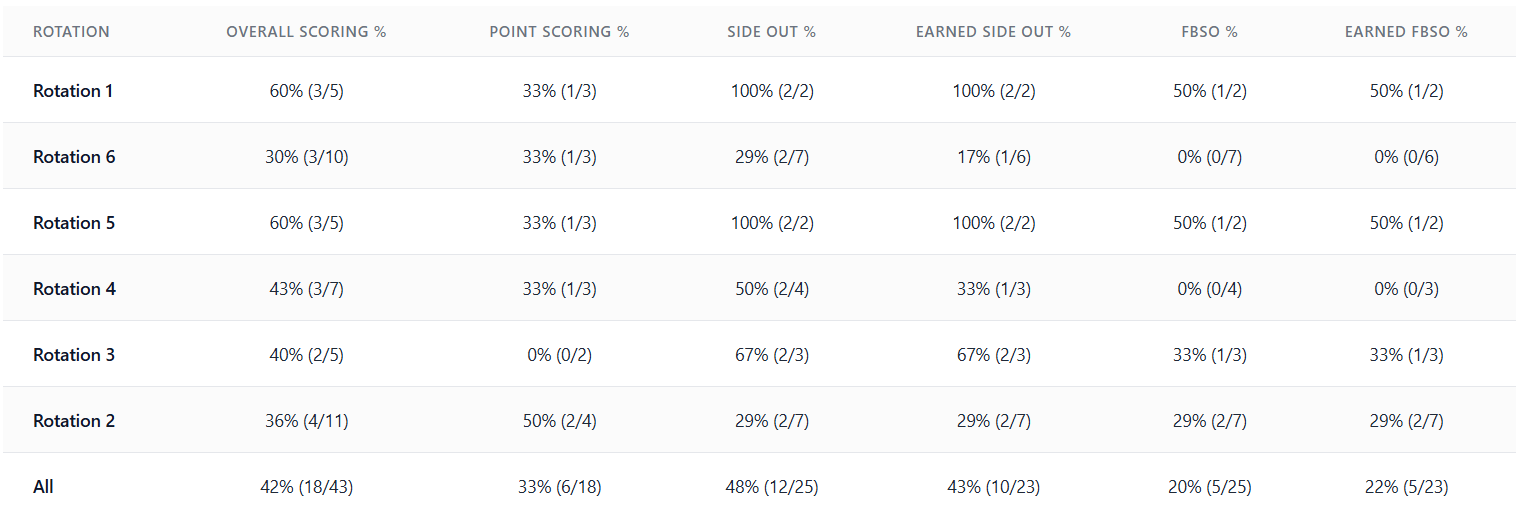
\includegraphics[width=\textwidth]{PL1_AM/SET2/ROT_STATS.png}
  \caption{\label{fig:PL1_ROT_STATS_2}Rotatie statistieken gemaakt door Balltime AI voor Lindemans Aalst in set 2.}
\end{figure}
